\section{Immagini}
Solitamente in un documento si ha la necessità di inserire delle immagini o 
per spiegare meglio il contenuto o per abbellire il testo. Per inserire le 
immagini in \LaTeX{} solitamente si utlizza il pacchetto \verb!\graphicx! 
(quindi nel preambolo è necessario inserire \verb!\usepackage{graphicx}!). Il 
comando da utilizzare è \verb!\includegraphics[opzioni]{img_path}!, dove le 
opzioni sono opzionali\footnote{No, non ci scusiamo per il gioco di parole} e 
le più comuni sono:
\begin{itemize}
    \item \textbf{width}: per la larghezza;
    \item \textbf{height}: per l'altezza;
    \item \textbf{scale}: per scalare l'immagine (1.0 è il 100\%);
    \item \textbf{keepaspectratio}: per mantenere lo stesso rapporto 
    larghezza-altezza dell’immagine originale
\end{itemize}
\verb!img_path! serve per specificare il percorso dell'immagine da includere, 
che può essere assoluto o relativo (meglio specificare il percorso relativo, 
specificare il percorso assoluto è un po' come passare per casa se devi andare 
dall'aula al bagno). È possibile anche specificare nel preabolo, tramite il 
comando \verb!\graphicspath{{default_path}}! il percorso di default per le 
immagini. In questo modo al posto di un percorso nel comando 
\verb!\includegraphic! è possibile passare il nome dell'immagine voluta.

Come per le tabelle abbiamo bisogno di un ``ambiente'' che contenga le 
immagini, che in questo caso sarà \verb!\begin{figure}...\end{figure}!.

È buona norma accompagnare le immagini con una didascalia che le spieghi. Per 
fare ciò ci viene in aiuto il comando \verb!\caption{...}! che accetta tra le 
parentesi graffe del testo per descrivere le immagini.

Attenzione! Non tutti i formati di immagini sono supportati! I formati 
supporti sono \textbf{pdf}, \textbf{png} e \textbf{jpg}. Nelle nuove 
installazioni di \LaTeX{} è possibile utilizzare però anche il formato \textbf{
eps}.

Di seguito possiamo vedere un esempio di come inserire un'immagine con 
didascalia in un documento \LaTeX{}.
\lstinputlisting{res/examples/esempioimmagine.tex}
Il risultato sarà questo:
\begin{figure}[H]
    \centering
    
\includegraphics[scale=0.15]{immagine}
    \caption{Didascalia dell'immagine}
\end{figure}


\subsection{Affiancare le immagini}
(Fate un respiro profondo che sennò qui si perde il proprio posto in paradiso) 
\\
Per poter affiancare immagini è possibile utilizzare il \textit{subfig} (Non è 
l'unica soluzione, ma è una delle più semplici). Questo permette di creare 
``delle piccole immagini'' all'interno dell'ambiente 
\verb!\begin{figure}...\end{figure}!. Specificando grandezza delle immagini o 
utilizzando i comandi per iniziare una nuova riga. È probabilmente più facile 
con un esempio.
\lstinputlisting{res/examples/esempio4immagini.tex}
Il risultato sarà questo:
\begin{figure}[H]
    \subfloat[Didascalia immagine 1]{
        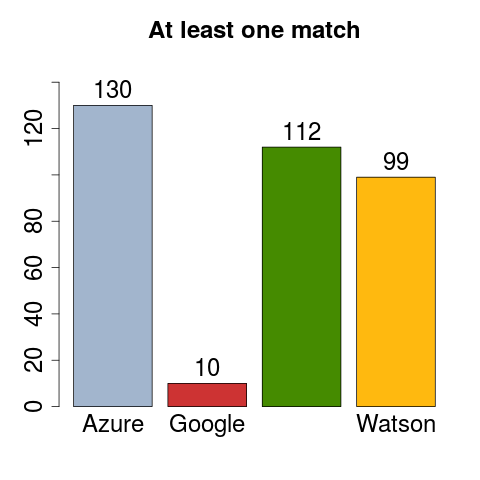
\includegraphics[width=0.45\linewidth]
        {immagine1}
    }
    \hfill
    \subfloat[Didascalia immagine 2]{
        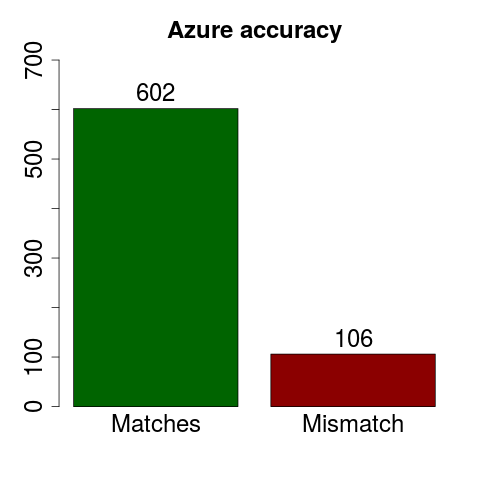
\includegraphics[width=0.45\linewidth]
        {immagine2}
    }
    \\
    \subfloat[Didascalia immagine 3]{
        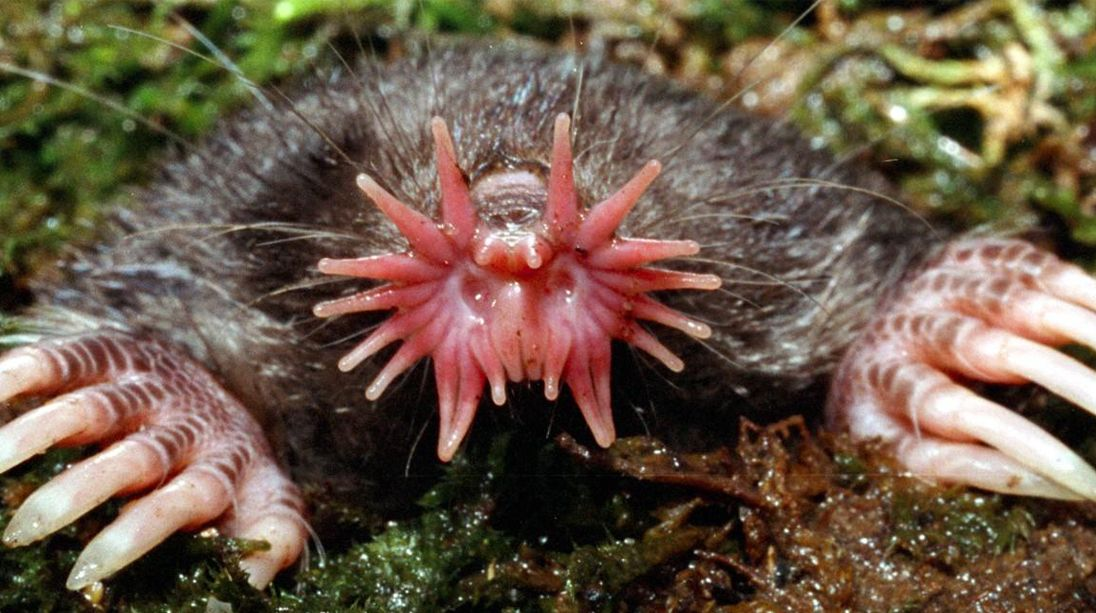
\includegraphics[width=\linewidth]
        {immagine3}
    }
    \\
    \subfloat[Didascalia immagine 4]{
        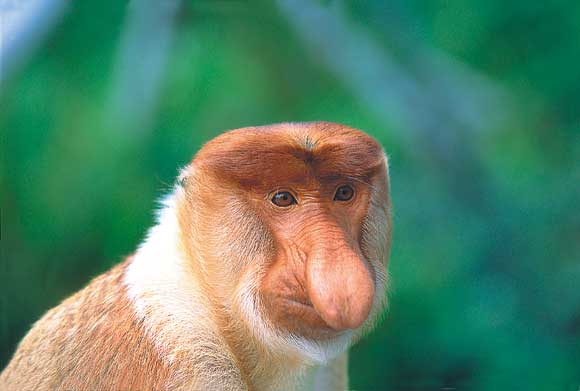
\includegraphics[width=0.60\linewidth]
        {immagine4}
    }
    \caption{Didascalia globale delle 4 immagini}
\end{figure}
Nell'esempio viene utilizzato il comando \verb!\subfloat! per posizionare le 
quattro immagini al quale, tra parentesi quadre, viene specificata la 
didascalia della singola immagine, mentre tra parentesi graffe viene indicata 
l'immagine da mostrare. Con il comando \verb!\caption! viene, infine, 
specificata la didascalia per le immagini raggruppate.

\subsection{Affiancare testo e immagini}
Sì si può anche affiancare testo e immagini. Serve? Bho vedete voi. In ogni 
caso è possibile utilizzando il \textit{package} \verb!wrapfig!. Questo 
funziona in modo analogo al solito modo di inserire le immagini, tranne che 
l'ambiente sarà \\
\verb!\begin{wrapfig}{pos}{dim}...\end{wrapfig}! dove \texttt{
pos} può essere \textbf{r} o \textbf{l} e \texttt{dim} serve per specificare 
le dimensioni di quanto l'immagine deve ``affiancarsi'' al testo. Di seguito 
un esempio. 
\lstinputlisting{res/examples/esempiotestoafianco.tex}
Il risultato sarà questo (è stato utilizzato il comando \texttt{lipsum} per 
mettere del testo riempitivo perchè non avevamo voglia di scrivere del testo 
sensato):
\newpage
\documentclass{article}
\usepackage{graphicx}
\usepackage{wrapfig}
\usepackage{lipsum}

\begin{document}
    \lipsum[1]
    \begin{wrapfigure}{r}{2cm}
        
\includegraphics[scale=0.2]{../img/immagine}
        \caption{Didascalia dell'immagine}
    \end{wrapfigure} 
    \lipsum[2-3]
\end{document}
\newpage

\section{Note a piè di pagina}
Spesso capita di dover mettere delle note a piè di pagina, per esempio per 
mettere un riferimento o spiegare meglio qualcosa\footnote{O solo per 
distrarre il lettore, come in questo caso.}. Per fare ciò è necessario 
utilizzare il comando \verb!\footnote{...}! specificando tra graffe il testo 
della nota. \LaTeX{} in automatico si occuperà della numerazione e del 
posizionamento.


\section{Collegamenti ipertestuali}

\subsection{Collegamenti nel testo}
Quando si inseriscono delle immagini e se ne fa riferimento nel testo oppure 
quando si scrive una parte e la si riprende in un'altra sezione del documento 
si sente la necessità di inserire un collegamento tra le due parti. Per fare 
ciò è necessario marcare con \verb!\label{...}! le parti a cui si vuole fare 
riferimento. Tra parentesi graffe deve essere inserito un identificativo 
univoco all'interno del documento che serve per indicare una specifica parte 
del documento o oggetto in esso. Quando ci si riferisce ad esso, invece, si 
deve utilizzare \verb!\ref{...}!, specificando tra graffe l'identificativo 
messo nella \verb!label!. È possibile anche fare riferimento alla pagina in 
cui si trova l'oggetto marcato con \verb!label! utilizzando 
\verb!\pageref{...}! (e lo stesso identificativo).

\subsubsection{Buone regole per gli identificativi}
Solitamente, agli identificativi utilizzati dalle \verb!label! e \verb!ref! 
vengono anteposti alcuni caratteri che permettono di identificare che tipo di 
oggetto è referenziato. 
\begin{table}[]
\centering
\begin{tabular}{ll}
\hline
\textbf{prefisso} & \textbf{tipologia}         \\ \hline
sec:              & section                    \\ \hline
subsec:           & subsection                 \\ \hline
fig:              & figure                     \\ \hline
tab:              & tabella                    \\ \hline
eq:               & formula                    \\ \hline
lst:              & codice                     \\ \hline
itm:              & elementi di lista numerata \\ \hline
alg:              & algoritmo                  \\ \hline
app:              & appendice                  \\ \hline
\end{tabular}
\end{table}
Questo non è difatto obbligatorio, ma è una buona regola, almeno per un motivo 
strettamente pratico: ci si ricorda a che tipo di oggetto ci si sta riferendo! 
Sembra sciocco ma quando si inizia ad avere un documento di svariate pagine, 
con, magari, anche solo un centinaio di pagine, fare confusione è veramente 
facile. Altro pericolo che si evita è l'avere etichette con lo stesso nome. 
(Siete stati avvertiti, fate come volete a vostro rischio e pericolo)


\subsection{Collegamenti al Web}
Il pacchetto che permette l'inserimento in maniera corretta in un documento \
LaTeX{} di \textit{link} o \textit{URL} è \verb!hyperref!. Ci sono due 
modalità principali per inserire queste informazioni. La prima è 
\verb!\url{indirizzo}!, con la quale verrà mostrato l'URL in formato \textit{
monospace}, pensato anche per documenti che devono essere stampati, la seconda 
è \verb!\href{indirizzo}{testo_da_mostrare}!, la quale non mostrerà 
esplicitamente l'indirizzo, ma mostrerà solamente il testo voluto (come 
succede nei siti Web per capirci), pensato per i documenti che devono 
essere fruiti in formato PDF. 

\subsubsection{Email}
Per inserire gli indirizzi email nel testo è preferibile creare questo comando 
personalizzato, da inserire nel preambolo del documento
\begin{lstlisting}
\newcommand{\mail}[1]{\href{mailto:#1}{\texttt{#1}}}
\end{lstlisting}
(per il momento fidatevi, spiegheremo in seguito come creare i propri 
comandi). L'utilizzo è molto semplice, infatti nel documento è sufficiente 
dare il comando \verb!\email{...}! specificando l'indirizzo di posta 
elettronica voluto.

\subsubsection{Personalizzazione dei link}
È buona norma, almeno nella creazione dei siti Web, colorare i link con un 
colore differente dal testo normale, in modo da evidenziare a chi visita la 
pagina che lì ci si può cliccare. Anche nei documenti non fa male evidenziare 
questi indirizzi e il pacchetto \verb!hyperref! permette la personalizzazione 
tramite il comando \verb!\hypersetup{...}! da mettere nel preambolo del 
documento, al quale devono essere specificate le personalizzazioni volute. Le 
più importanti sono:
\begin{itemize}
    \item \textbf{colorlinks=false} oppure \textbf{colorlinks=true}, che 
    indica rispettivamente se si vuole che i link vengano riquadrati oppure 
    colorati;
    \item \textbf{urlcolor=color} che serve per specificare il colore dei link 
    (sostituite \textit{color} con un colore in lingua inglese);
\end{itemize}
Maggiori informazioni possono essere reperite nel capitolo 
\href{https://en.wikibooks.org/wiki/LaTeX/Hyperlinks}{Hyperlinks} su WikiBook 
(oppure come abbiamo imparato prima all'URL 
\url{https://en.wikibooks.org/wiki/LaTeX/Hyperlinks} così abbiamo anche un 
esempio dei due modi di inserire i collegamenti ai siti).